\chapter{Existující algoritmy pro kompresi XML}
\label{kapitolaXmlAlgoritmy}

Velikost XML dokumentu danou vlastností formátu, kdy se schéma opakuje pro každý záznam, lze při kompresi redukovat pomocí například gzip\footnote{GNU zip, software pro kompresi dat využívající LZ77 a Huffmanovo kódování.}. Jiným přístupem může být navržení kompresního algoritmu speciálně pro XML. Algoritmy využívající znalost vnitřní struktury XML se anglicky nazývají XML aware. Díky této znalosti dokážou data před\-při\-pra\-vit tak, aby byla komprese co nejefektivnější. Pro kompresi samotnou jsou používány algoritmy již zmiňované v kapitolách \ref{kapitolaStatistickaKomprese} a \ref{kapitolaSlovnikovaKomprese} a jejich upravené varianty.

XML aware algoritmy můžeme rozdělit dle několika kritérií a to zda podporují dotazování a přístup do komprimovaných dat nebo zda je či není dekompresní algoritmus závislý na přístupu k XML schématu. Z druhé skupiny je častější použití algoritmů, které jsou na schématu nezávislé, protože pro dekompresi není vždy možné přístup ke schématu zaručit.

\section{XMill}
\label{xmill}
Algoritmus XMill, který nepodporuje dotazování do zkomprimovaných dat, představili pánové Hartmut Liefke a Dan Suciu v roce 2000. Jeho architektura využívá knihovnu kompresních algoritmů zlib, specifické kompresory pro určitý typ dat a navíc podporuje použití kompresorů vytvořených uživatelem pro speciální typy dat. Rozhodnutí, který kompresní algoritmus bude použit, je provedeno na základě znalosti tagů. Architektura algoritmu XMill je postavena na třech základních principech \cite{xmill}:

\begin{itemize}
\item Struktura XML složená z tagů a atributů tvoří strom. Data, obsah elementů a hodnoty atributů jsou reprezentovány jako řetězce. Stromová struktura a data jsou komprimovány odděleně.
\item Datové položky stejných elementů jsou seskupeny do jednoho kontejneru a každý kontejner je komprimován odděleně.
\item Dle typu dat (text, číslo apod.) je pro kompresi kontejneru použit vhodný kompresní algoritmus, tzv. sémantický kompresor.
\end{itemize}

\subsection{Popis architektury}
Architektura algoritmu XMill je zobrazena na obrázku \ref{architekturaXMill}. XML dokument je nejprve zpracován pomocí SAX\footnote{Simple API for XML.} parseru, který každý prvek pošle do Path procesoru. Path procesor rozhodne, do kterého existujícího kontejneru prvek vloží nebo zda má vytvořit kontejner nový. Ke každému kontejneru může být uživatelem přiřazen sémantický kompresor a to buď atomický implementovaný v XMill, kombinace atomických pro komplexnější typy, nebo vlastní. Kontejnery jsou plněny až do předem určené velikosti (defaultně je to 8~MB), je-li tato velikost dosažena, je kontejner zkomprimován pomocí gzip, uložen na disk a komprese dále pokračuje. Díky tomu jsou data rozdělena do vzájemně nezávislých bloků.

\begin{figure}[!htb]
\centering
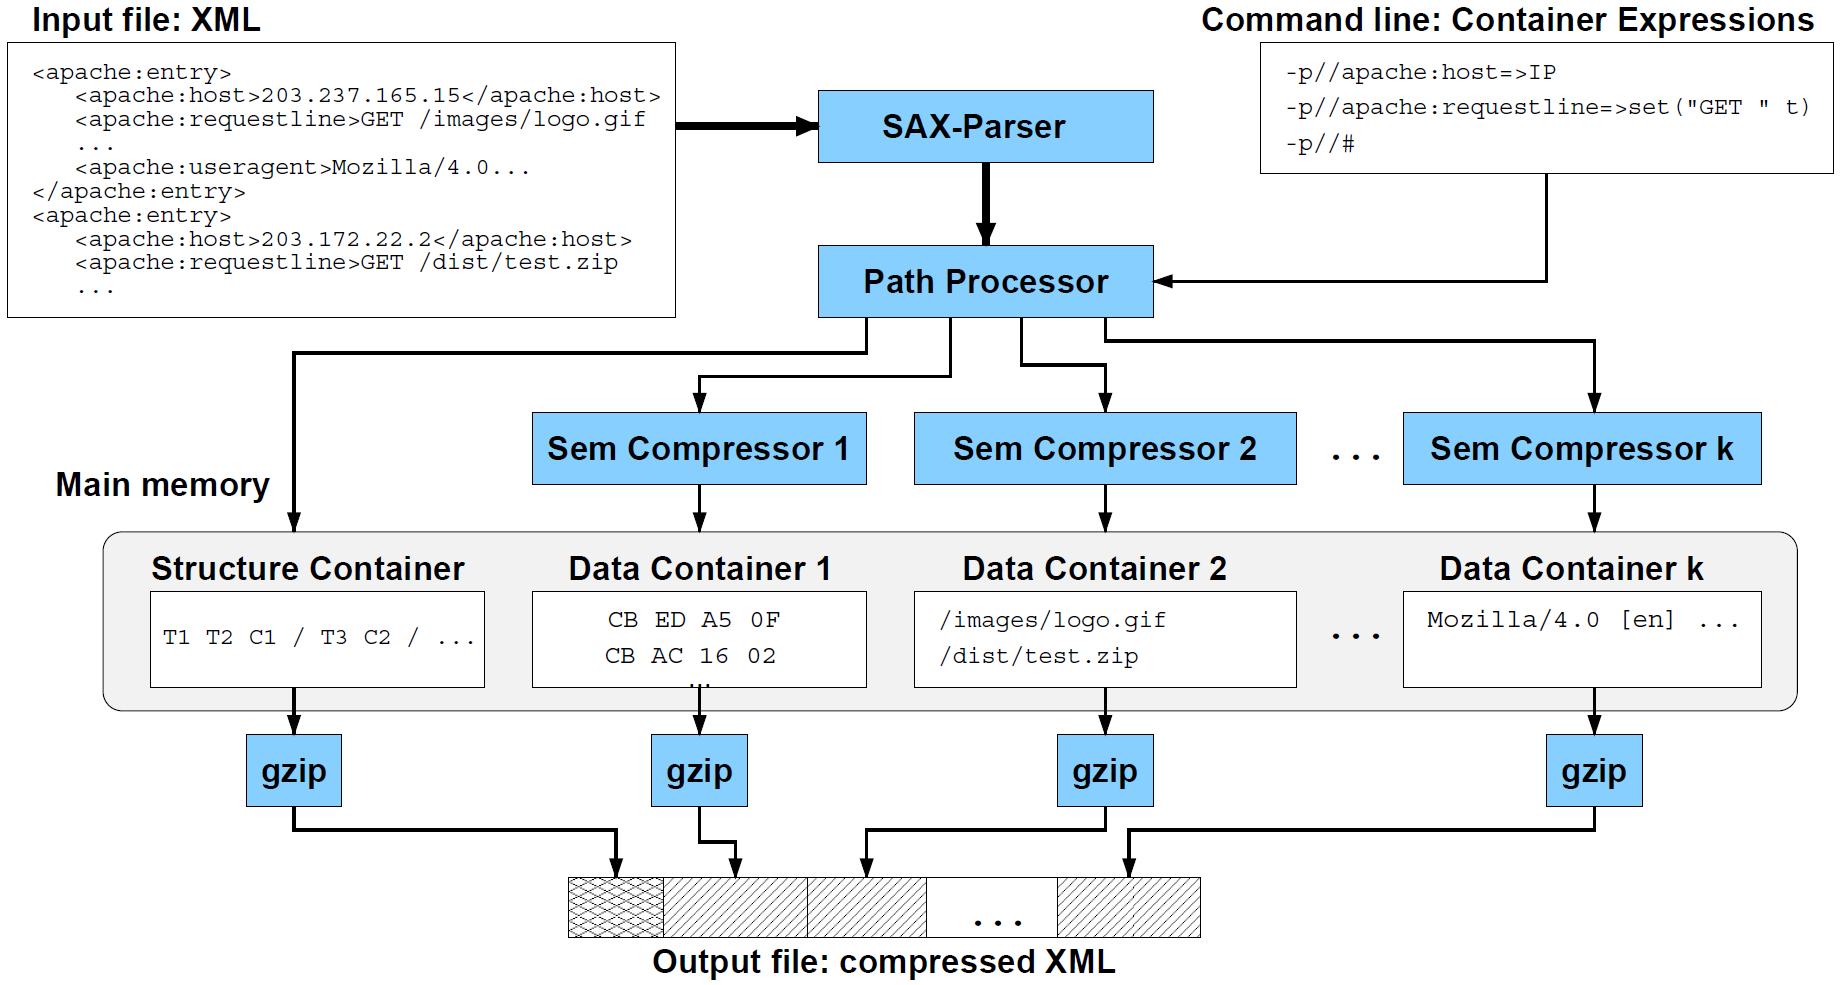
\includegraphics[clip, angle=0, width=150mm]{ArchitekturaXMill}
\caption{Architektura algoritmu XMill \cite{xmill}}
\label{architekturaXMill}
\end{figure}

\subsection{Oddělení struktury od dat}
\label{xmillOddeleniStruktury}
Struktura XML je složena z tagů a atributů. Počáteční tagy a atributy jsou kódovány slovníkovou metodou a nahrazeny indexem ve slovníku, kladným celým číslem. Ukončující tag je kódován hodnotou 0, při dekompresi je díky syntaxi zřejmé, který tag je ukončován. Datové hodnoty jsou nahrazeny záporným indexem kontejneru, do kterého byly přiřazeny. \cite{xmill}

Pro příklad zpracujeme následující informace o článku:

\begin{verbatim}
<article mdate="2011-01-11" key="journals/acta/GoodmanS83">
  <author>
    <name>Nathan Goodman</name>
    <title>Mr.</title>
  </author>
  <title>NP-complete Problems Simplified on Tree Schemas.</title>
</article>
\end{verbatim}

Tagy zde jsou \texttt{article}, \texttt{author} a \texttt{title} a atributy \texttt{mdate} a \texttt{key}. Po zpracování dostaneme výstup \texttt{1 2 -3 3 -4 0 4 5 -5 0 6 -6 0 0 7 -7 0 0}. Lze si povšimnout, že indexování kontejnerů začíná až číslem 3, to proto, že index 0 je rezervován pro kontejner struktury, 1 pro kontejner bílých znaků (umožňuje zachování formátovacích mezer) a 2 pro kontejner obsahující procesní instrukce, DTD a jiné.

\subsection{Seskupení dat stejného významu}
Mapování mezi daty a kontejnery provádí Path procesor na základě cesty k datům (path) a~na uživatelem definovaném regulárním výrazu container expression. Základní myšlenkou je hodnotám pro každý tag nebo atribut přiřadit vlastní kontejner. Cesta k datům v~příkladě z předchozí části \ref{xmillOddeleniStruktury} vypadá například  pro atribut takto \texttt{/article/@key} a~pro tag takto \texttt{/article/author/name}. Pomocí container expression je možné nastavit pravidla, kdy budou například hodnoty různých tagů ukládány do stejného kontejneru. \cite{xmill}

\subsection{Sémantická komprese}
Jak již bylo zmíněno v úvodu popisu tohoto algoritmu, jsou podporovány 3 druhy sé\-man\-ti\-ckých kompresorů: atomické, kombinované a definované uživatelem. Atomických kompresorů je 8, například textový kompresor \texttt{t}, který řetězec pouze zkopíruje na výstup (ten bude později zkomprimován pomocí gzip), nebo kompresor \texttt{u}, který komprimuje kladná celá čísla.

Kombinovaný kompresor je vhodný pro hodnoty, ve kterých lze nalézt nějaký vzor nebo strukturu. Jako příklad lze uvést sekvenční kompresor pro kompresi IP adresy \texttt{seq(u8 "." u8 "." u8 "." u8)}, což znamená sekvenci čtyř kladných celých čísel menších než 256 oddělených tečkou.

Vlastní kompresory lze s výhodou použít na data, která mají strukturu složitou nebo velmi těžce vyjádřitelnou pomocí kombinovaných kompresorů. Autoři jako příklad takových dat uvádějí DNA sekvence. Aby bylo možné data komprimovaná za pomoci vlastních kompresorů zpětně rekonstruovat, musí mít dekompresní algoritmus samozřejmě také přístup k~použitému vlastnímu kompresoru. \cite{xmill}

\subsection{Nedostatky tohoto přístupu}
Způsob rozdělení struktury a dat různých typů zvlášť do jednotlivých bloků v algoritmu XMill brání úpravě komprimovaných dat nebo efektivnímu dotazování nad nimi. Možnost dotazů nad daty je ale pro některé aplikace velmi důležitá a v případě algoritmů typu LZ nebo XMill by to znamenalo zbytečně náročnou operaci: dekomprimovat data, provést dotazy nebo úpravy a data zpět zkomprimovat.

\section{XGrind}
\label{xgrind}
Na základě výše zmíněných požadavků publikovali pánové Pankaj M. Tolani a Jayant R. Haritsa v roce 2002 článek, ve kterém představili nový kompresní nástroj, který přímo podporuje dotazování nad zkomprimovanými daty. Ten, namísto rozdělení struktury celého dokumentu, komprimuje obsah jednotlivých elementů a atributů pomocí semiadaptivního Huffmanova kódování (viz \ref{huffmanovoKodovani}), které je nezávislé na kontextu.

Díky tomu podporuje dotazy typu úplná shoda nebo shoda prefixu tak, že je dotaz zakódován pomocí stromu vytvořeného při kompresi, následně jsou ve zkomprimovaném souboru vyhledána data odpovídající dotazu a pouze ta jsou dekomprimována a zobrazena uživateli. To odpovídá nejmenšímu možnému objemu dat, který je nutný dekomprimovat. Algoritmus navíc podporuje i intervalové dotazy a dotazy na podřetězec, ty ale vyžadují částečnou dekompresi příslušných elementů či atributů. \cite{xgrind}

\subsection{Kompresní techniky}
\label{xgrindKompresniTechniky}
Způsob kódování tagů a atributů je velice podobný jako v případě algoritmu XMill (viz \ref{xmillOddeleniStruktury}). Každý počáteční tag je kódován jako zřetězení \texttt{T} a unikátního indexu tagu. Podobně jsou atributy kódovány zřetězením \texttt{A} a unikátního indexu atributu. Koncové tagy jsou kódovány symbolem \texttt{/}, což je možné díky syntaxi. Výčtové typy, jejichž definice je uvedena v DTD nebo ve schématu dokumentu, jsou kódovány pomocí schématu $\log_2n$, kde $n$ je počet prvků výčtového typu.

Aby bylo možné se efektivně dotazovat do komprimovaných dat, je pro kompresi hodnot elementů a atributů použito kompresní schéma, které řetězci přiřadí kód nezávislý na místě výskytu v dokumentu. To splňuje použité semiadaptivní Huffmanovo kódování (viz \ref{huffmanovoKodovani}), které ve dvou průchodech nejprve vytvoří kódy na základě statistiky a poté data zakóduje. V algoritmu XGrind nejsou kódovány jednotlivé znaky, ale celé hodnoty, které spolu sémanticky souvisejí. \cite{xgrind}

Zakódujme nyní zkrácenou verzi příkladu k algoritmu XMill:
\begin{verbatim}
<article mdate="2011-01-11">
    <author>
        <name>Nathan Goodman</name>
    </author>
    <title>NP-complete Problems</title>
</article>
\end{verbatim}

Výstupem bude sekvence \texttt{T0 A0 }\textit{huff}(\texttt{2011-01-11})\texttt{ T1 T2 }\textit{huff}(\texttt{Nathan Goodman})\texttt{ / / T3 }\textit{huff}(\texttt{NP-complete Problems})\texttt{ / /}, kde je výrazem \textit{huff}(\texttt{A}) myšlen semiadaptivní Huffmanův kód řetězce \texttt{A}.

\subsection{Popis architektury}
Schéma architektury lze vidět na obrázku \ref{architekturaXGrind}, jehož originální verze byla publikována v~\cite{xgrind}. Hlavní prvkem je XGrind Kernel, který nejprve vyzve DTD-Parser k načtení DTD a inicializaci Frequency Tables naplněním všemi unikátními tagy a nevýčtovými atributy a Symbol Table naplněním výčtovými atributy. Následně XGrind Kernel vyzve \mbox{XML-Parser} k přečtení zpracovávaného dokumentu a naplnění Frequency Tables statistikou počtu výskytů jednotlivých prvků. Nakonec XGrind Kernel znovu vyzve XML-Parser, aby vytvořil zakódovanou (viz \ref{xgrindKompresniTechniky}) podobu XML dokumentu. \cite{xgrind}

\begin{figure}[!htb]
\centering
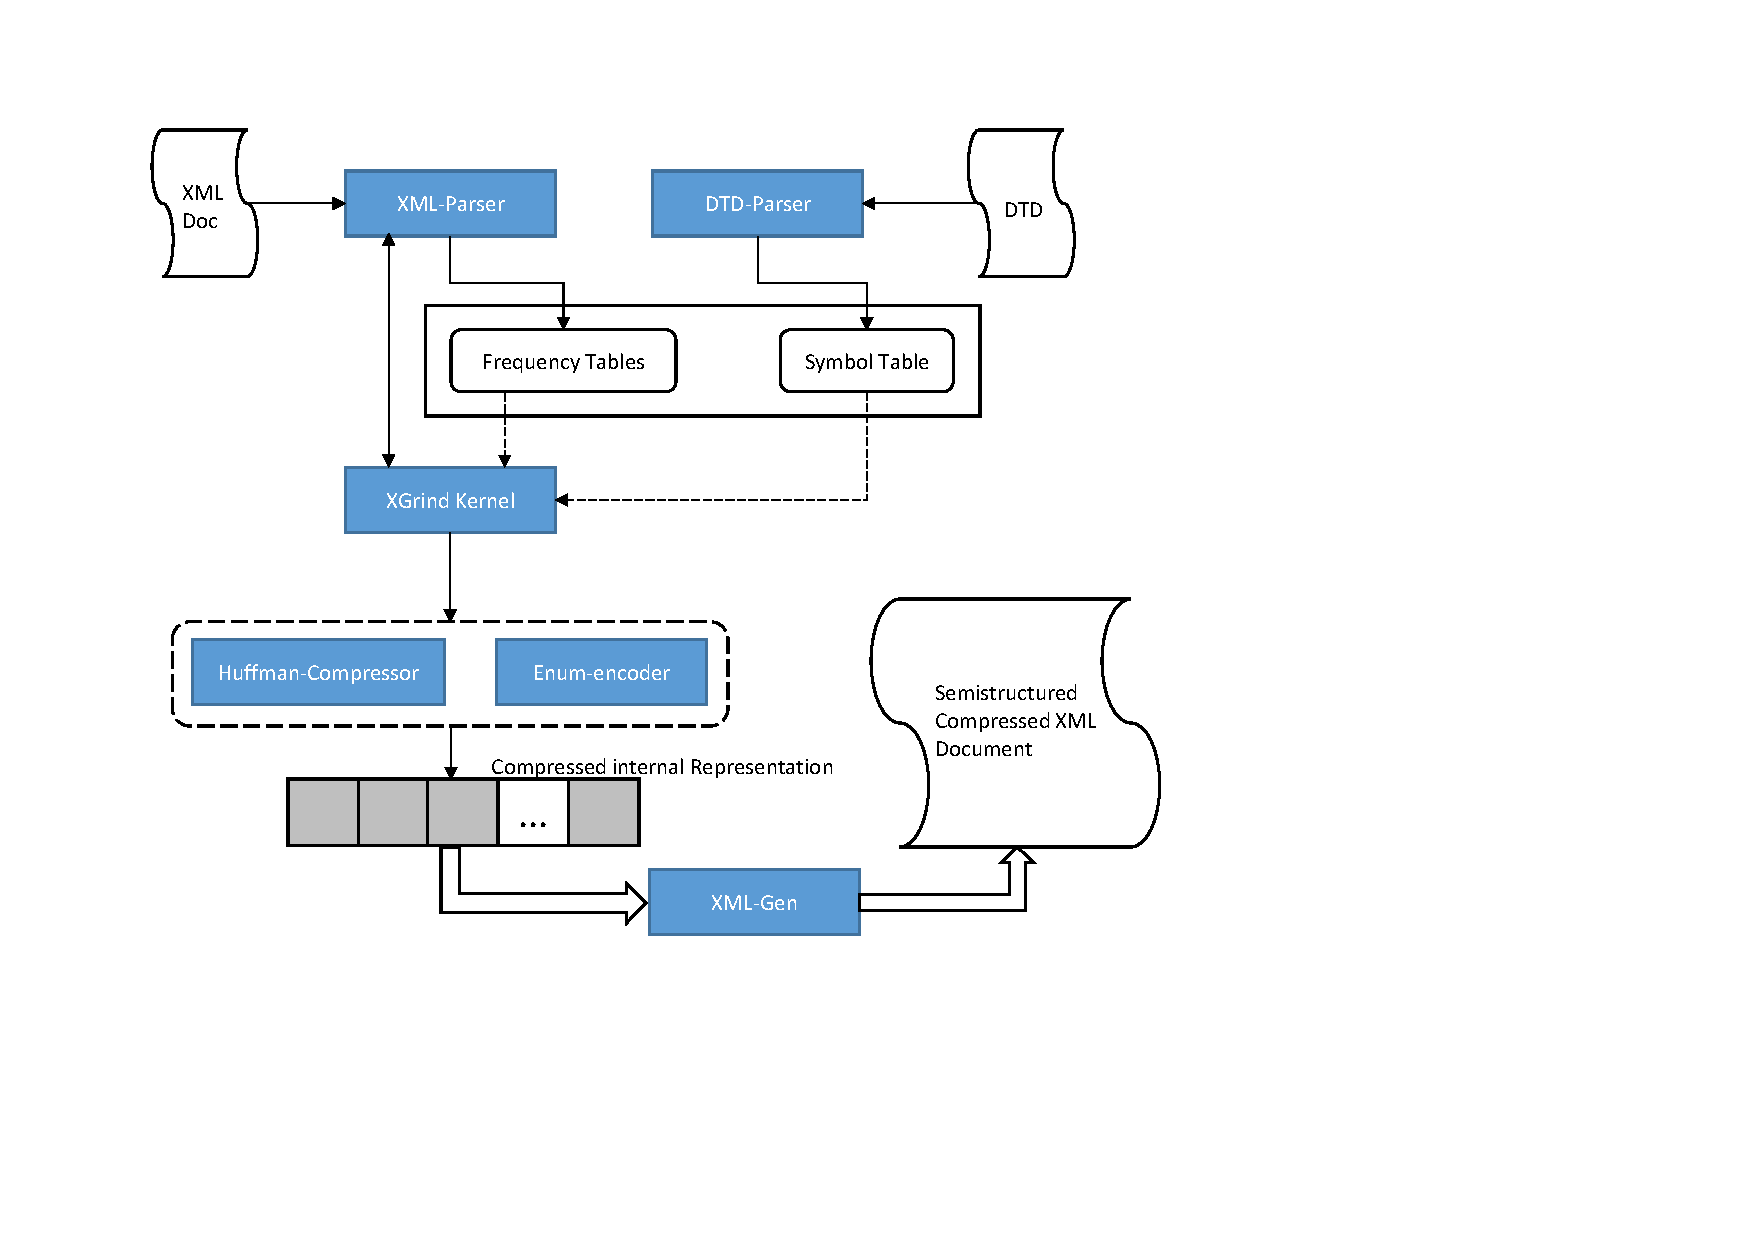
\includegraphics[trim=70 150 284 60, clip, angle=0, width=150mm]{xgrindArchitektura}
\caption{Architektura algoritmu XGrind}
\label{architekturaXGrind}
\end{figure}

\subsection{Dotazování}
Zpracování dotazů je implementováno pomocí slovníkového analyzéru, který poskytuje kódy tagů, atributů a hodnot, a parserem, který se stará o vzájemné porovnávání dotazu s daty. Parser prochází XML dokument do hloubky jako strom a uchovává si informaci o~místě (cesta), kde v dokumentu se právě nachází, a obsah uzlů, které právě zpracovává.

Pro dotazy na přesnou a prefixovou shodu jsou zakódovány cesta a dotaz a při hledání jsou data označena jako vyhovující dotazu pouze v případě, že požadovaná cesta odpovídá aktuální pozici parseru v zakódovaných datech a zakódovaná verze dotazu odpovídá obsahu uzlu. Pro dotazy na rozsah nebo částečnou shodu musí být data ve vybraných uzlech dekomprimována a porovnání je provedeno na jejich původních verzích. \cite{xgrind}